% Frontpage - Titlingpage from Memoir class 
\begin{titlingpage}
  
  \thispagestyle{empty}
  
  % Define the colourbar on the frontpage
  \begin{tikzpicture}[remember picture,overlay]
    \coordinate [below=2.5cm] (midpoint) at (current page.north);

    \node [name=colourbar,
    anchor=base,
    fill=ase_blue,
    text = white,
    minimum width=\paperwidth,
    minimum height=1cm] at (midpoint) {\logoHuge{\textsc{{Aarhus School Of
            Engineering}}}};

    % Define the point where the logo will go
    \coordinate [right=4cm] (ase_logo) at (colourbar.west);

    % Set coordinate system origin
    \begin{scope}[shift=(ase_logo)]
      % Draw the outline
      \filldraw [white] (1.2,0.85) -- (-1.6,0.85) -- (-2.3,-0.85) -- (1.2,-0.85) --cycle;
      % Include the logo
      \node [xshift=-0.5cm]{\includegraphics[width=3cm]{ase_logo.png}};
    \end{scope}
  \end{tikzpicture}

  % Temporary center margins
  \begin{adjustwidth}{-0.5cm}{0cm}
    \vspace*{\stretch{0.5}}
    \centering
    { \setlength{\baselineskip}{32pt}
      {\SuperHuge \stext{Auto-OMA on Wind Turbine Hub} 
      }\par
      \stext{<Subtitle Example : Implemented on a Andriod system>}
      \par\vspace*{4\onelineskip}
      \par
      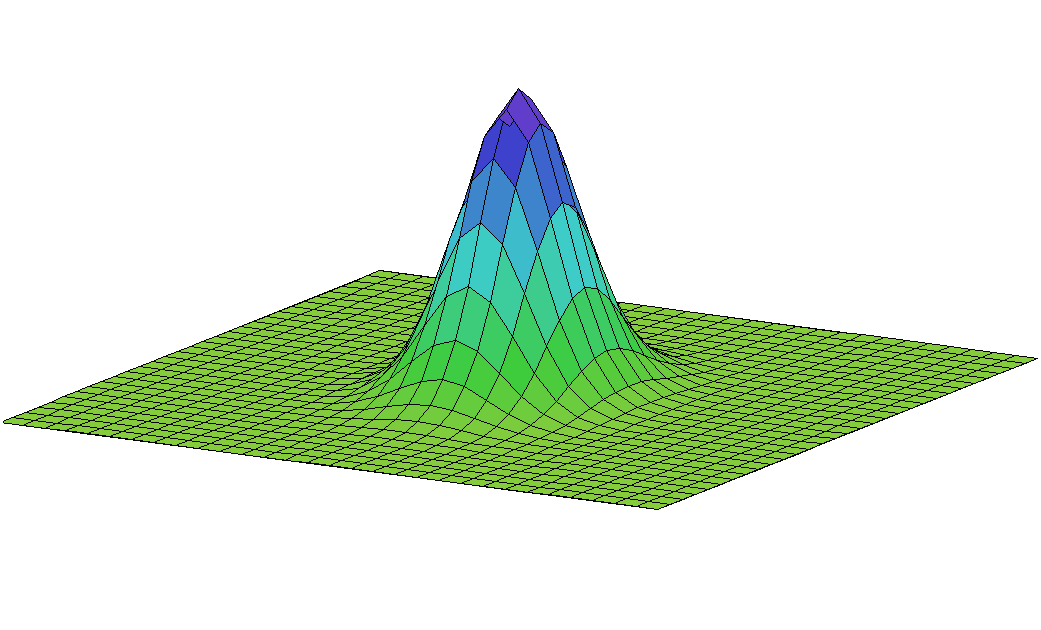
\includegraphics[width=10cm]{frontpage}
      \par\vspace*{4\onelineskip}
      \textbf{\stext{Master Thesis}}\par
      \vspace{-0.5cm}
      \textbf{\stext{Structural Engineering}}\par
      \par\vspace*{2\onelineskip}
      % Make a table to make the --- align
      \stext{Anders Olsen}\par
      \vspace{-0.5cm}
      \stext{11495}\par
    }
    \vfill
    \begin{tabular}{l l c r}
    \stext{Supervisors:}	& \stext{Peter Olsen}	&	\hspace{2.5cm}		&	\stext{June $25^{\text{th}}$, 2017}\\
    									&	\stext{Martin \O rum \O rhem Juul}	&	\hspace{2.5cm}	&	\\
	\end{tabular}
    \enlargethispage{3.5\onelineskip}
  \end{adjustwidth}
\end{titlingpage}







